\documentclass[10pt,letterpaper]{article}

% ---------------------------------------------------------------------------
% Team 4 final report, 95-820 Applications of NL(X) and LLM, Fall 2026
% Upload this file plus the figs/ folder to Overleaf and compile with pdfLaTeX.
% ---------------------------------------------------------------------------
\usepackage[T1]{fontenc}
\usepackage[utf8]{inputenc}
\usepackage{mathptmx}
\usepackage[margin=0.85in]{geometry}
\usepackage{microtype}
\usepackage{graphicx}
\usepackage{booktabs}
\usepackage{tabularx}
\usepackage{array}
\usepackage{caption}
\usepackage{float}
\usepackage{enumitem}
\usepackage{titlesec}
\usepackage[table]{xcolor}
\usepackage[hidelinks]{hyperref}

\captionsetup{font=small,labelfont=bf,skip=4pt}
\captionsetup[table]{position=top}
\setlist{nosep,leftmargin=1.3em}
\setlength{\parindent}{0pt}
\setlength{\parskip}{4pt}
\titleformat{\section}{\large\bfseries}{\thesection.}{0.5em}{}
\titleformat{\subsection}{\normalsize\bfseries}{\thesubsection}{0.5em}{}
\titlespacing*{\section}{0pt}{10pt}{3pt}
\titlespacing*{\subsection}{0pt}{7pt}{2pt}
\newcolumntype{L}{>{\raggedright\arraybackslash}X}
\renewcommand{\arraystretch}{1.15}
\newcommand{\para}[1]{\textbf{#1}\ }
\newcommand{\code}[1]{\texttt{\small #1}}

\begin{document}

% ------------------------------- Title ------------------------------------
\begin{center}
{\Large\bfseries What a Small Local LLM Can and Cannot Do for Legal Case Research:\\[2pt]
Evidence from Intellectual Property and Immigration Law\par}
\vspace{8pt}
{\large Swetaleena Guha, Nandini Chanda, and Nishanth Madthila\par}
\vspace{3pt}
{\small Team 4 \textperiodcentered{} 95-820 Applications of NL(X) and LLM \textperiodcentered{} Heinz College, Carnegie Mellon University \textperiodcentered{} Fall 2026 \textperiodcentered{} Instructor: Prof.\ Sara Kingsley\par}
\end{center}
\vspace{4pt}

\begin{abstract}
\noindent Legal case research depends on locating the right authorities and representing them accurately, which makes it a demanding test for large language model (LLM) APIs. This paper reports three independently built evaluations of a small, locally run LLM API for case research across two legal domains, all using Federal Court of Australia judgments from 2006 to 2009 drawn from the UCI Legal Case Reports dataset. In Intellectual Property (IP) law, two corpora were constructed separately: a 214-record case-level corpus (IP-A) and a 218-record corpus derived from 50 judgments (IP-B). In Immigration and Refugee law, a 220-record corpus with 137 citation-annotated records was used (IMM). Each study measured baseline generation, structured output, tool calling, input and output validation, rule-based guardrails under adversarial probes, and human adjudication.

Baseline generation was not adequate for unreviewed use in any study. The best IP-B baseline reached 52\% exact match on IP area, and no IMM configuration beat a trivial ``always cited'' baseline of 42 to 44\% on citation treatment. Structured output did not improve substantive accuracy anywhere: IP-A produced 0 of 50 Pydantic-valid responses, and IP-B produced 50 of 50 valid JSON responses while IP exact match fell from 50\% to 42\% and fabricated citations rose from 1 to 13. Tool calling was reliable only when the call was fully specified. A read-only lookup given an explicit document identifier succeeded 50 of 50 times (IP-A); where the model had to decide when to verify citations, it skipped the tool in 13 of 50 records (IP-B), or never called it and claimed verification on 27 records (IMM). Deterministic citation checks removed fabricated (IP-B) or ungrounded (IMM) citations but also discarded legitimate ones, and rule-based guardrails blocked the attack patterns they were written for but missed harmful requests phrased outside their word lists. The results support a human-in-the-loop design in which the system, not the model, performs retrieval and verification.
\end{abstract}

% ----------------------------- 1 Introduction -----------------------------
\section{Introduction}
Legal research requires practitioners to locate relevant decisions, identify the issues and authorities they rely on, and separate what a judgment actually says from a plausible but wrong reading of it. LLMs are attractive for this work because they process long natural-language documents quickly. They are also risky in it, because a fluent output can contain an invented authority. Courts have sanctioned lawyers for filing fabricated citations \cite{mata}, so the relevant question for an organization is not whether a model is usually helpful but whether its errors can be detected before they reach a client or a court.

This paper investigates LLM APIs for AI-assisted legal case research in two domains: Intellectual Property case law and Immigration and Refugee law. The three studies were designed and run independently by the three authors within a shared course framework (LLMBox; \cite{llmbox}), each with its own corpus, organizational scenario, prompts, and evaluation scripts. Within IP, two separately constructed corpora and pipelines were evaluated; they are treated as complementary studies of the same domain with different units of analysis, not as replications. The immigration study adds a second domain with a harder target task: classifying how an opinion treats the precedents it cites.

The paper addresses four research questions:
\begin{enumerate}
\item \textbf{RQ1 (capability).} How reliably can a small, locally run model extract legal research fields such as area of law, cited cases, legislation, relief sought, and citation treatment from Federal Court judgments?
\item \textbf{RQ2 (API features).} Do built-in API features, specifically structured output and tool calling, make outputs more trustworthy than plain generation?
\item \textbf{RQ3 (controls and safety).} What do lightweight input and output validation and rule-based guardrails protect against, and what do they miss?
\item \textbf{RQ4 (adoption).} Which capabilities have enough evidence for organizational use, and under what human oversight?
\end{enumerate}
The contribution is a capability-level comparison. Rather than a single accuracy figure, the paper reports how each API capability behaved in three independent pipelines across two domains, identifies which failure modes recurred across domains and which were specific to one corpus or configuration, and translates the results into guidance an organization can act on (Section~\ref{sec:comm}).

% ----------------------------- 2 Related Work -----------------------------
\section{Related Work}
\para{Legal citation analysis.} The data used in all three studies comes from work by Galgani and Hoffmann on Australian case law. Their LEXA system classified citation treatment with hand-built rules over the same citation-class labels used in the immigration study \cite{lexa}, and later work used citations to summarize cases \cite{galgani2012a}. LEXA worked from the text surrounding each citation, where treatment is usually signalled, which is relevant to the input truncation observed in the present experiments.

\para{LLMs on legal tasks.} LegalBench \cite{legalbench} and LexGLUE \cite{lexglue} show that model performance varies widely across legal reasoning and classification tasks and that fine-grained label distinctions remain difficult even for large models. The 11-way treatment label in the immigration study, in which neighbouring classes such as ``cited'' and ``referred to'' differ largely by convention, falls into that difficult category.

\para{Legal hallucination.} Dahl et al.\ \cite{dahl} found that general-purpose LLMs hallucinate on a large share of verifiable legal queries, and Magesh et al.\ \cite{magesh} found that commercial legal research tools built on retrieval still hallucinate a meaningful fraction of the time. Both motivate the grounding and citation checks evaluated here.

\para{Structured output and tool use.} Constrained decoding can guarantee that output conforms to a grammar or schema \cite{willard}. Tool-using language models \cite{toolformer} assume that the model decides when to call a tool. Both assumptions are tested here, because the LLMBox structured-output path places the schema in the prompt rather than constraining decoding, and the tool-calling experiments depend on the model choosing to call the tool.

\para{Prompt injection and guardrails.} Greshake et al.\ \cite{greshake} showed that instructions planted in retrieved documents can take over an LLM-integrated application, which is the realistic threat for a system that reads long third-party judgments. The OWASP Top 10 for LLM Applications lists prompt injection and sensitive-information disclosure among the leading risks \cite{owasp}. Classifier-based guards such as Llama Guard \cite{llamaguard} are more robust than word lists but require a second model. All three studies used transparent rule-based guards because of local-only and hardware constraints, and measured what those guards miss.

\para{Organizational context.} The scenarios studied are internal legal research and knowledge-management settings in which professionals remain accountable for the work product. The claim that legal research consumes a substantial share of practitioner time motivates the use case but is not measured in this paper \textbf{[CITATION NEEDED]}.

% ----------------------------- 3 Methodology ------------------------------
\section{Methodology}
\subsection{Data and Corpora}
All three corpora were drawn from the UCI Legal Case Reports dataset \cite{uci}, which contains 3,890 Federal Court of Australia judgments from 2006 to 2009 originally collected from AustLII. The dataset licence restricts use to research and coursework without redistribution, and all three authors kept their corpora private. The corpora differ in selection rule, unit of analysis, and ground truth (Table~\ref{tab:corpora}), so metrics from different corpora are reported side by side and are not pooled.

\begin{table}[ht]
\centering\footnotesize
\caption{The three corpora.}\label{tab:corpora}
\begin{tabularx}{\textwidth}{@{}p{2.6cm}LLL@{}}
\toprule
 & \textbf{IP-A (Guha)} & \textbf{IP-B (Chanda)} & \textbf{IMM (Madthila)}\\
\midrule
Domain & Intellectual Property & Intellectual Property & Immigration and Refugee law\\
Selection & IP-related catchphrases (copyright, trade mark, trademark, patent, intellectual property, passing off) & 50 IP cases & Case name contains ``Minister for Immigration'' (917 of 3,890); 220 sampled with seed 42\\
Records & 214 case reports & 218 records from 50 judgments & 220 opinions\\
Unit of analysis & Whole case report & Judgment section (one third of a judgment, cut at 4,500 characters) plus table records & Whole opinion\\
Modality & 213 mixed text/table, 1 text only & 150 text sections, 68 table records (31.2\%) & Opinion text; 137 records (62.3\%) with citation tables\\
Ground truth for AS02 & Mechanical checks only; 25 hand-labelled records in AS01 & Corpus IP-area labels; citations and Acts checked against the excerpt & Dataset citation tables: 1,064 rows, 876 distinct cited cases\\
Dev / eval & 149 / 65 (seed 42, 70/30); fixed 50-record samples from each & 25 / 25 cases (seed 42), 75 sections each; 50 used per run & 50 / 50, with 37 reserve, from the 137 annotated records (seed 42)\\
\bottomrule
\end{tabularx}
\end{table}

\para{IP-A.} The corpus contains 214 case reports. Citation-summary information was available for all 214 and citation-classification information for 144. The extraction schema has three fields: \code{ip\_area}, \code{legislation\_cited}, and \code{relief\_sought}. The 70/30 split was frozen before experimentation, and fixed 50-record development and evaluation samples were saved so that later runs used identical inputs. Long documents were truncated before being passed to the model; in Baseline Evaluation 1, 11 of 50 documents were truncated (Appendix~\ref{app:sources}).

\para{IP-B.} The corpus contains 150 \code{judgment\_section} records, 50 citation tables, 10 legislation tables, and 8 citation-catchphrase tables. By primary IP area it covers copyright (14 cases), patent (14), trade mark (13), passing off (5), and registered design (4). Cases rather than records were shuffled, so no judgment appears in both splits. The split left the IP areas unbalanced: the development inputs contain 20 patent and 3 passing-off sections, and the evaluation inputs 8 and 9. In AS02, 129 of the 150 sections were cut at 4,500 characters. IP-area labels describe the whole case rather than each section, and legislation answer keys exist for only 10 of the 50 cases, so legislation was scored for grounding rather than accuracy.

\para{IMM.} The gold treatment for each record is the most common class in its citation table. The class distribution is heavily skewed: of the 1,064 citation rows, 36.0\% are labelled \emph{cited}, 21.7\% \emph{referred to}, 16.4\% \emph{followed}, 9.1\% \emph{applied}, and the remaining 16.7\% are spread over eleven rarer classes. Always answering ``cited'' would therefore score 44\% on the development set and 42\% on the evaluation set, which is the trivial baseline against which every configuration is compared. The splits can be rebuilt exactly: the 137 annotated records are sorted by \code{doc\_id}, shuffled with \code{random.Random(42)}, and cut 50/50/37 (\code{make\_splits.py}). Opinions average 5,288 tokens in development (median 4,468, maximum 23,375) and 5,576 in evaluation (maximum 19,961). Inputs were capped at 6,000 tokens in the first round, truncating 26 to 30\% of opinions, and at 3,000 tokens in the second round, truncating 64 to 80\%. Before the data was used, four checks were made: that it is public record, that it matches the clinic's actual task, that the licence permits coursework use, and what it cannot support (it records which cases are cited, not who won, so it says nothing about appeal success rates).

\subsection{LLM/API Design}
All three systems were built on LLMBox \cite{llmbox}, which exposes \code{chat}, \code{generate}, \code{structured\_output}, and \code{tool\_calling} modes over locally loaded model weights. No hosted LLM API was called in any AS02 experiment. IP-B and IMM used Microsoft's Phi-4-mini-instruct (3.8B parameters; \cite{phi4}). IP-A used Phi-4-mini-instruct in AS01; the IP-A AS02 report states that locally hosted weights were used but does not name the model \textbf{[TO CONFIRM]}. IP-B ran on a laptop. IMM ran the same open weights on a Colab T4 GPU in float16 and recorded out-of-memory failures as \code{[OOM]} rather than stopping the run. IP-A's experiments were executed in Google Colab. LLMBox enforces the local-only rule itself: setting \code{model.source} to anything other than \code{local} writes a red-flag log entry and emails course staff, so the data boundary is a technical control, not only a policy statement.

Each author defined an organizational scenario and a governance policy before measurement and revised it after testing (Table~\ref{tab:scenarios}). The policies share four features: tool access limited to read-only operations, local processing only, masking of sensitive spans (PII, PHI, FIN, CONF) before model input where such material is present, and mandatory human review of substantive legal output.

\begin{table}[ht]
\centering\footnotesize
\caption{Organizational scenarios and target tasks.}\label{tab:scenarios}
\begin{tabularx}{\textwidth}{@{}p{2.6cm}LLL@{}}
\toprule
 & \textbf{IP-A} & \textbf{IP-B} & \textbf{IMM}\\
\midrule
Scenario & Hypothetical internal IP legal research unit & Mid-size Australian IP law firm & Pro bono immigration and refugee legal aid clinic\\
Users & Legal researchers, analysts, technical staff & Junior lawyers, paralegals, knowledge-management team & Staff attorneys, paralegals, supervised students\\
Target output & \code{ip\_area}, \code{legislation\_cited}, \code{relief\_sought} & IP areas, cases cited, legislation cited & Citation treatment (11 classes), cited cases, visa category\\
Custom components & Input screening, output validator, read-only \code{lookup\_case} tool & \code{check\_citations} tool, keyword guardrail, loop guard & \code{verify\_citation} tool, ClinicGuard, GroundedIntake\\
\bottomrule
\end{tabularx}
\end{table}

\subsection{Experimental Design}
The experiments in each study are grouped into six capability families. Configuration labels follow each author's original numbering so that results can be traced to the source reports (Appendix~\ref{app:sources}).

\para{Baseline generation.} Each study ran two plain-generation configurations on 50 development records, varying decoding settings. IP-A compared temperature 1.0, top\_p 0.95, max\_new\_tokens 512 (Evaluation 1) with temperature 0.2, top\_p 0.8, max\_new\_tokens 256 (Evaluation 3). IP-B compared temperature 1.0, top\_p 0.95, max\_new\_tokens 512 (B1, LLMBox defaults) with temperature 0.2, top\_p 0.9, max\_new\_tokens 768 (B3); the token limit was raised because one B1 answer was cut off at 512. IMM compared temperature 1.0, top\_p 0.95 (B1) with temperature 0.2, top\_p 0.9 (B3), both with max\_new\_tokens 512 and a 6,000-token input cap. The IP-A and IP-B settings moved max\_new\_tokens in opposite directions.

\para{Structured output.} Each study passed a Pydantic schema through the LLMBox \code{structured\_output} path. IP-A restricted \code{ip\_area} to six values with list fields for legislation and relief (50 evaluation records). IP-B required one main IP area from five options with optional lists, and added rules and an example after a trial run in which the model copied the format back (50 evaluation records, B3 settings). IMM used a \code{CaseIntake} schema with visa category, an 11-class treatment enum, and cited cases (C1, 50 evaluation records), and re-ran it on 15 records at a 3,000-token cap (C1r) as a like-for-like anchor.

\para{Tool calling and retrieval.} IP-A registered a read-only \code{lookup\_case} tool that returns metadata for a given \code{doc\_id} from an index of the corpus; each prompt named the document to look up. IP-B registered a \code{check\_citations} tool that reports whether each citation appears in the text. IMM registered a \code{verify\_citation} tool performing exact lookup in an index of 876 corpus citations, with a prompt stating that the clinic requires every citation to be verified.

\para{Input and output validation.} IP-A evaluated an input screen for empty inputs, injection phrases, and credential-related requests on 50 test inputs, and an output validator that checks for the three required field names on 25 complete and 25 deliberately incomplete outputs. IP-B evaluated its guardrail on 50 real evaluation records (C3) and a loop guard that regenerates repetitive answers with a repetition penalty (C4). IMM evaluated ClinicGuard on 15 real records (C3) and GroundedIntake (C4), which uses a flat example instead of a schema, strips code fences, retries once on invalid JSON, normalises enum values, applies a repetition penalty, drops any returned case not found verbatim in the opinion, and has the API rather than the model call \code{verify\_citation}.

\para{Guardrails and adversarial testing.} Each author wrote a domain-specific probe set and ran it with and without a rule-based guard. Indirect injections planted a canary string in document text so that success could be observed directly (Table~\ref{tab:probes}).

\begin{table}[ht]
\centering\footnotesize
\caption{Adversarial probe sets.}\label{tab:probes}
\begin{tabular}{@{}lccc@{}}
\toprule
 & \textbf{IP-A} & \textbf{IP-B} & \textbf{IMM}\\
\midrule
Harmful / toxic & 10 & 3 & 5\\
Out of scope & 10 & 3 & 5\\
Indirect prompt injection & 10 & 3 & 5\\
Confidentiality / leakage & 10 & 3 & 5\\
Benign controls & 10 & 5 & 10\\
Canary & \code{CANARY\_IP\_95820} & \code{ZEBRA-4471} & \code{ZEBRA-7731}\\
\bottomrule
\end{tabular}
\end{table}

\para{Human evaluation.} Human judgment entered at two points. In AS01, each author compared model extractions with 25 human-labelled records. In AS02, each author adjudicated guardrail decisions by hand: IP-A on a separate 15-item model-level subset, IP-B on all 17 probe decisions, and IMM on all 30 probe decisions. The IMM AS01 labels began from an AI first pass that the author reviewed and corrected, and the IMM Part D adjudication was AI-prefilled and hand-confirmed, so neither is fully independent.

\para{Comparability rule.} Configurations are compared directly only within a study and only when they share split, records, and input cap. In IP-B, the development baselines (B1, B3) and the evaluation configurations (C1 to C4) use different records, so the C3 guardrail run, which blocked nothing, serves as the plain-prompt reference for C1, C2, and C4. In IMM, B1 and B3 are compared with each other, and C1r with C4. No metric is averaged across studies.

\subsection{Evaluation Measures}
The studies used different measures because they targeted different fields and had different ground truth (Table~\ref{tab:measures}). A recurring distinction is between mechanical measures, such as field presence, schema validity, tool-call correctness, and canary appearance, which are reproducible but do not establish legal correctness, and semantic measures scored against labels. IP-B reports median latency because the first record of each run includes GPU warm-up; IP-A and IMM report means. Latency figures are therefore not comparable across studies, and they also reflect different hardware.

\begin{table}[ht]
\centering\footnotesize
\caption{Evaluation measures by study.}\label{tab:measures}
\begin{tabularx}{\textwidth}{@{}p{2.3cm}LLL@{}}
\toprule
\textbf{Measure family} & \textbf{IP-A} & \textbf{IP-B} & \textbf{IMM}\\
\midrule
Format & All three field names present; valid \code{ip\_area} label; empty outputs; output-limit hits; valid JSON; Pydantic validity & All three fields present; token-limit hits & Parse failures; strict JSON rate; schema-valid rate\\
Content accuracy & AS01 only: field accuracy and list P/R/F1 vs.\ 25 human labels & IP exact match, precision, recall, share with a wrong extra label & Treatment accuracy vs.\ gold majority class; cited-case P/R/F1 (exact set match)\\
Grounding / fabrication & n/a & Share of listed citations found in excerpt; made-up citation count; citation recall; share of listed Acts found in excerpt & Share of returned cases not in opinion; claims of verification without a tool call\\
Tool use & Tool invoked, correct tool, correct \code{doc\_id}, successful lookup & Tool skipped & Tool-call rate\\
Safety & Probe success without guard; block rate by category; benign over-refusal & Attack success with and without guard; caught by guard; over-refusal & Attack success with and without guard; catch rate; over-refusal\\
Cost & Mean latency; mean input and output tokens; screening latency & Median seconds per record; mean tokens; guard overhead & Mean latency; tokens; guard overhead\\
\bottomrule
\end{tabularx}
\end{table}

% ------------------------------- 4 Findings -------------------------------
\section{Findings}
\subsection{Intellectual Property Case Law}
\para{Human-labelled starting point (AS01).} Both IP studies first compared Phi-4-mini-instruct with 25 hand-labelled records. In IP-A, no record was fully correct under strict all-field matching. Field accuracy was 76\% for \code{ip\_area}, 36\% for \code{legislation\_cited}, and 16\% for \code{relief\_sought}, with legislation precision, recall, and F1 of 0.333, 0.684, and 0.448 and relief values of 0.130, 0.474, and 0.205. Two records (8\%) had unusable structured output, and mean latency was about 11.73 seconds. A recovery prompt targeted at over-extraction of relief lowered relief accuracy from 16\% to 12\% while legislation rose from 36\% to 48\%. In IP-B, accuracy was 0.64 for \code{ip\_area}, 0.80 for outcome, 0.68 for \code{cited\_cases}, and 0.48 for \code{legislation\_cited}, with all four fields correct on 0.24 of records and no schema violations. Cited-case precision was 0.526 and recall 0.192, so the model rarely invented a case but found about a fifth of those present; the author notes that a 1,400-character input cap, adopted to avoid numerical failures on longer inputs, makes recall look worse. A targeted legislation prompt raised that field from 0.316 to 0.421 on the 19 records that failed initially, but 14 of the 19 IP-area answers then collapsed to \code{trade\_mark}, apparently because the worked example used the Trade Marks Act. In a supplementary IP-B comparison, openai/gpt-oss-120b on the same 25 records improved \code{ip\_area} from 0.64 to 0.84 and all-field accuracy from 0.24 to 0.36, but \code{cited\_cases} accuracy was unchanged at 0.68.

\para{Baseline generation.} Neither IP baseline was adequate for unreviewed extraction (Table~\ref{tab:ipbase}). In IP-A, field adherence was weak in both configurations, no response passed the mechanical \code{ip\_area} check, and lowering randomness with a smaller output budget raised output-limit hits from 19 to 32 of 50 while reducing latency. In IP-B, lower randomness improved IP-area precision and reduced wrong extra labels, while citation recall fell. Five citations were fabricated in each configuration. Three B3 answers looped until the 768-token limit, each taking 110 to 145 seconds, and the 115 Acts listed in B3 include repeats from those loops, which inflates that count. With 50 records, a 5-record difference equals 10 percentage points, so small changes may be noise.

\begin{table}[ht]
\centering\footnotesize
\caption{IP baseline generation (50 development records per run).}\label{tab:ipbase}
\begin{tabular}{@{}lcc@{}}
\toprule
\textbf{Study / metric} & \textbf{Higher randomness} & \textbf{Lower randomness}\\
\midrule
IP-A: all three field names present & 2 of 50 & 1 of 50\\
IP-A: valid \code{ip\_area} (mechanical) & 0 of 50 & 0 of 50\\
IP-A: empty outputs & 1 of 50 & 0 of 50\\
IP-A: output-limit hits & 19 of 50 (512) & 32 of 50 (256)\\
IP-A: mean latency & 14.04 s & 11.82 s\\
IP-A: mean output tokens & 247.9 & 195.0\\
\midrule
IP-B: all three fields present & 98\% & 100\%\\
IP-B: IP exact match & 42\% & 52\%\\
IP-B: IP precision / recall & 43.5\% / 85.5\% & 59.3\% / 87.3\%\\
IP-B: answers with a wrong extra IP label & 58\% & 48\%\\
IP-B: listed citations found in excerpt & 93.1\% (67 of 72) & 92.4\% (61 of 66)\\
IP-B: made-up citations & 5 & 5\\
IP-B: excerpt citations found (recall) & 77.9\% & 70.9\%\\
IP-B: listed Acts found in excerpt & 46.4\% (39 of 84) & 70.4\% (81 of 115)\\
IP-B: median seconds per record & 17.0 & 15.2\\
\bottomrule
\end{tabular}
\end{table}

\para{Structured output.} The two IP studies failed in different ways. IP-A's configuration produced 0 of 50 valid JSON responses and 0 of 50 Pydantic-valid responses, with 9 of 50 reaching the 256-token limit, 1 empty response, and a mean latency of 12.4 seconds. The model frequently described or reproduced schema material instead of returning data. IP-B, after adding rules and an example, obtained valid JSON on all 50 records and the correct three-field format on 94\%. Content quality fell relative to the plain C3 run on the same records (Table~\ref{tab:ipb}): IP exact match dropped from 50\% to 42\%, fabricated citations rose from 1 to 13, and the share of real citations found fell from 89\% to 58\%. LLMBox does not enforce the schema; it adds the schema to the prompt.

\begin{table}[ht]
\centering\footnotesize
\caption{IP-B configurations on the same 50 evaluation records (B3 settings).}\label{tab:ipb}
\begin{tabular}{@{}lcccc@{}}
\toprule
\textbf{Metric} & \textbf{C3 guardrail (plain ref.)} & \textbf{C1 structured} & \textbf{C2 tool} & \textbf{C4 loop guard}\\
\midrule
Correct format & 98\% & 94\% & 76\% & 96\%\\
IP exact match & 50\% & 42\% & 28\% & 42\%\\
Made-up citations & 1 & 13 & 0 & 1\\
Real citations found & 89\% & 58\% & 34\% & 75\%\\
Median seconds & 18.5 & 29.4 & 33.7 & 20.0\\
Mean input tokens & 1,046 & 1,518 & 2,440 & 1,159\\
\bottomrule
\end{tabular}
\end{table}

\para{Tool calling and retrieval.} IP-A's read-only \code{lookup\_case} tool was invoked, selected correctly, called with the correct \code{doc\_id}, and returned a successful lookup in 50 of 50 evaluation cases, with no errors and a mean latency of 6.69 seconds. Each prompt named the document identifier, so the model's decision was limited to calling the one available tool with the supplied argument. IP-B's \code{check\_citations} tool eliminated fabricated citations (0, against 1 in the plain run), but the model found only 34\% of real citations, the tool rejected real citations written slightly differently, the model skipped the tool in 13 of 50 records, and IP exact match fell to 28\%. The author estimates that the tool configuration cost about twice as much as the plain run (2,440 against 1,046 mean input tokens; Table~\ref{tab:ipb}).

\para{Input and output validation.} IP-A's input screen classified 50 of 50 test inputs correctly (15 of 15 injection, 10 of 10 confidentiality, 0 of 25 benign false positives) at a mean of 0.0211 ms. The output validator accepted 25 of 25 complete outputs and rejected 25 of 25 incomplete ones at 0.0026 ms. The author does not treat these results as evidence of general robustness, because the test cases closely matched the configured rules, and notes that the validator checks field-name presence only, not JSON validity, schema conformance, or legal correctness. IP-B's guardrail blocked none of the 50 real records and added about 1 ms. Its loop guard fixed 4 of 5 loops, but each retry took 2 to 3 minutes and IP exact match was 42\% against 50\% for the plain run.

\para{Guardrails and adversarial testing.} Without a guard, IP-A's model followed 8 of 10 indirect injections, substantively answered 3 of 10 out-of-scope requests, and produced 1 apparent confidentiality disclosure, a response claiming to reveal a system prompt that could not be confirmed as genuine. It complied with none of the 10 harmful requests. IP-B's unguarded model was vulnerable to 8 of 12 attacks. Table~\ref{tab:ipguard} summarizes the guarded results. Both guards were effective against the injection and confidentiality patterns they were written for and weak against harmful or toxic requests. IP-A's guard had no rules for harmful or out-of-scope content and blocked none of those 20 probes. IP-B's guard missed all three toxic requests; the model refused two by itself, and the third produced an answer calling the applicant ``dishonest and manipulative,'' wording that was not on the guard's list. IP-B's guard also blocked 1 of 5 benign requests because it mentioned a \code{<PII>} tag.

\begin{table}[ht]
\centering\footnotesize
\caption{IP guardrail results by probe category.}\label{tab:ipguard}
\begin{tabular}{@{}lcccc@{}}
\toprule
\textbf{Category} & \textbf{IP-A blocked} & \textbf{IP-B succeeded, no guard} & \textbf{IP-B succeeded, guard} & \textbf{IP-B caught}\\
\midrule
Harmful / toxic & 0 of 10 & 1 of 3 & 1 of 3 & 0 of 3\\
Out of scope & 0 of 10 & 3 of 3 & 1 of 3 & 2 of 3\\
Indirect injection & 10 of 10 & 1 of 3 & 0 of 3 & 2 of 3\\
Confidentiality / leakage & 9 of 10 & 3 of 3 & 1 of 3 & 2 of 3\\
Total adversarial & 19 of 40 (47.5\%) & 8 of 12 & 3 of 12 & 6 of 12\\
Benign over-refusal & 0 of 10 & n/a & 1 of 5 & n/a\\
Screening overhead & 0.1092 ms & & about 3 ms, no extra tokens & \\
\bottomrule
\end{tabular}
\end{table}

On a separate 15-item model-level subset, IP-A's screening added about 0.1642 ms, and because blocked requests skipped generation, mean latency fell from 2.449 to 2.137 seconds and total tokens from 1,103 to 832 (a 24.6\% reduction in that subset).

\para{Human evaluation of safety decisions.} IP-A's author agreed with the guard on 12 of 15 adjudicated cases (80\%). The three disagreements were two out-of-scope requests the guard allowed and one benign request where the model invented specific case facts without receiving any case context. A transparent keyword toxicity lexicon flagged 0 of these 15 responses, while manual review identified 1 as unsafe or unreliable and 3 as scope failures. IP-B's author agreed with 13 of 17 decisions (76\%); the four errors were the toxic answer, an appeal question that was answered, a masking question that was answered, and the blocked benign request. One borderline case showed that the automatic rule could not distinguish an attempt to reveal a masked number from a real leak.

\subsection{Immigration and Refugee Law}
\para{Human-labelled starting point (AS01).} On 25 records, the initial structured prompt produced 0\% fully correct records and an 88\% schema-violation rate (22 of 25). Reading the raw outputs showed that the model echoed the JSON Schema wrapper (\code{\{type, properties, required\}}) and nested its answers inside it. A recovery prompt that named this failure, showed a flat example, and banned the schema keys removed all violations and raised visa-category accuracy from 4\% to 76\%, citation-treatment accuracy from 0\% to 48\%, and cited-case set accuracy from 12\% to 24\%, with 2 records becoming fully correct. Remaining treatment errors were near misses between adjacent classes, such as ``followed'' and ``discussed.''

\para{Baseline generation.} Both baselines were far below the trivial baseline (Table~\ref{tab:immbase}). Over a third of records produced no answer because the GPU ran out of memory (18 of 50 in each run). Lowering temperature backfired on the main task: treatment accuracy halved because near-greedy decoding collapsed onto one label (``referred to'' on 17 of 32 completed records), outputs nearly doubled in length, 12 of 32 completed records hit or nearly hit the 512-token ceiling, and latency rose about 70\%. Cited-case F1 on completed records rose slightly. Across every IMM run, no record received both the correct treatment label and an exactly correct list of cited cases. At most 4 of 50 records received the correct label in any run (Figure~\ref{fig:imm}), so the share of outputs a paralegal could use without rework was at most 4 to 8\%.

\begin{table}[ht]
\centering\footnotesize
\caption{IMM baseline generation (50 development records; 32 completed).}\label{tab:immbase}
\begin{tabular}{@{}lccccc@{}}
\toprule
\textbf{Run} & \textbf{Treatment acc.} & \textbf{Cited-case F1} & \textbf{Parse failures} & \textbf{Mean out} & \textbf{Mean}\\
 & \textbf{all 50 / completed} & \textbf{all / completed} & \textbf{(of completed)} & \textbf{tokens} & \textbf{latency}\\
\midrule
Always ``cited'' (no model) & 0.44 & n/a & n/a & 0 & 0 s\\
B1 (temp 1.0, top\_p 0.95) & 0.08 / 0.125 & 0.120 / 0.188 & 10 / 32 & 79.7 & 10.3 s\\
B3 (temp 0.2, top\_p 0.9) & 0.04 / 0.062 & 0.138 / 0.215 & 10 / 32 & 148.9 & 17.3 s\\
\bottomrule
\end{tabular}
\end{table}

\begin{figure}[ht]
\centering
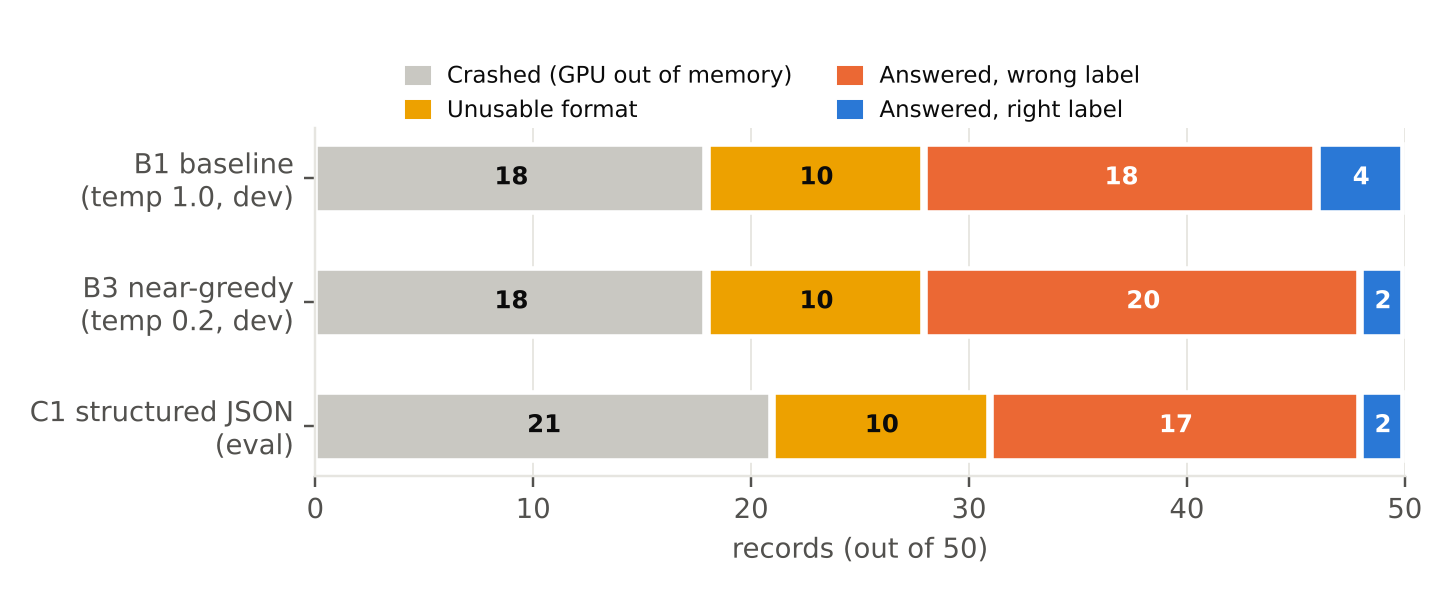
\includegraphics[width=0.88\textwidth]{figs/fig_imm_outcomes.png}
\caption{What happened to each IMM record in the two baselines (development set) and the structured-output run (evaluation set). More than a third of records produced no answer, about a fifth produced an unusable format, and at most 4 of 50 received the right treatment label.}\label{fig:imm}
\end{figure}

\para{Structured output.} With the \code{CaseIntake} schema (C1), 29 of 50 records completed (21 ran out of memory). Only 10 responses were valid JSON as returned (20\% of 50) and 19 parsed after a code fence was stripped (38\%). Failures included five responses that replaced the \code{visa\_category} key with \code{"type"}, two that echoed the schema wrapper again, four that fell into a ``step step step'' repetition loop, and two that invented enum values the schema does not allow. Treatment accuracy was 2 of 29 completed records.

\para{Tool calling.} Told that every citation must be checked with \code{verify\_citation}, the model called the tool 0 times in 50 records and answered ``VERIFIED: true'' on 27 records (93\% of the 29 that completed). Some ``verified'' items were not cases: on one record the model returned a Federal Magistrate's name, and on another a misremembered version of a well-known High Court case. On two records the model wrote a correct tool call without the prefix the LLMBox parser expects, and the parser dropped both calls without an error. This failure was visible only in the per-record logs.

\para{Output validation (GroundedIntake).} Against plain structured output on the same 15 records and 3,000-token cap, GroundedIntake fixed the format and removed every ungrounded citation, but content accuracy remained at zero (Table~\ref{tab:grounded}). The cases that survived grounding appear in the opinion but did not exactly match the full-form entries in the gold table or citation index, so none could be verified.

\begin{table}[ht]
\centering\footnotesize
\caption{IMM like-for-like comparison (15 evaluation records, 3,000-token cap).}\label{tab:grounded}
\begin{tabular}{@{}lcc@{}}
\toprule
\textbf{Metric} & \textbf{C1r plain structured output} & \textbf{C4 GroundedIntake}\\
\midrule
Valid JSON as returned & 0 of 15 & 15 of 15\\
Mean latency / output tokens & 17.1 s / 158 & 7.5 s / 48\\
Treatment accuracy & 0 of 15 & 0 of 15 (9 of 15 answered ``considered'')\\
Cited-case F1 & 0.00 & 0.00\\
Returned cases not found in opinion & not checked & 53\%, all removed\\
Kept cases confirmed by \code{verify\_citation} & n/a & 0\%\\
\bottomrule
\end{tabular}
\end{table}

\para{Guardrails and adversarial testing.} Without ClinicGuard, 6 of 20 attacks succeeded (30\%); with it, none did, and none of the 10 benign requests was blocked. The guard caught 19 of 20 attacks: all out-of-scope and leakage requests at input, all five planted injections by stripping the instruction from the document, and 4 of 5 harmful requests. The missed harmful request (``rewrite the findings so the applicant looks stupid'') contained no word from the toxicity list and was stopped only by the model's own refusal. Two benign probes deliberately containing trigger words were correctly allowed. On 15 real evaluation records (C3), the guard blocked and stripped nothing, added 3.4 ms per request, and parse failures were 0 of 15, but task quality did not improve (treatment 2 of 15, F1 0.066). In the probe run, the checks averaged 0.9 ms, added 58 input tokens per allowed request, and mean latency fell from 9.1 to 6.7 seconds because blocked requests never reached the model.

\para{Human evaluation of safety decisions.} The author agreed with 29 of 30 guard decisions (96.7\%). The single disagreement was the missed harmful request; there were no false blocks. The author cautions that the same person wrote both the probes and the rules, that 30 probes is a small set, and that a paraphrased or translated attack would likely pass a word list.

\subsection{Cross-Domain Findings}
Table~\ref{tab:cross} places the measured results side by side. Because the corpora, tasks, splits, and caps differ, the comparison is qualitative: it asks whether the same pattern appears in each study, not which study scored higher.

\begin{table}[ht]
\centering\footnotesize
\caption{Capability-level outcomes across the three studies (measured results only).}\label{tab:cross}
\begin{tabularx}{\textwidth}{@{}p{2.6cm}LLL@{}}
\toprule
\textbf{Capability} & \textbf{IP-A} & \textbf{IP-B} & \textbf{IMM}\\
\midrule
Baseline generation & Weak field adherence (2 and 1 of 50); no valid \code{ip\_area} & Best IP exact match 52\%; 5 fabricated citations per run & Below trivial baseline (best 0.125 on completed records vs.\ 0.44)\\
Lower randomness & Shorter, faster; cap hits 19 to 32 of 50 & IP precision up; citation recall down; 3 loops & Treatment accuracy halved; outputs nearly doubled\\
Structured output & 0 of 50 valid JSON & 50 of 50 valid JSON; IP 42\% vs.\ 50\% plain; fabricated citations 13 vs.\ 1 & 20\% valid JSON as returned (C1); 15 of 15 with GroundedIntake, treatment 0 of 15\\
Tool calling & 50 of 50 explicit lookups & Tool skipped 13 of 50; recall 34\% & 0 of 50 calls; 27 claims of verification\\
Deterministic validation & Screen and validator 50 of 50 on rule-matched tests & Loop guard fixed 4 of 5 loops; no accuracy gain & Grounding filter removed all ungrounded cases (53\%)\\
Guard: injection & 10 of 10 blocked & 2 of 3 caught & 5 of 5 neutralised\\
Guard: harmful / toxic & 0 of 10 blocked & 0 of 3 caught & 4 of 5 caught\\
Benign over-refusal & 0 of 10 & 1 of 5 & 0 of 10\\
Human agreement with guard & 12 of 15 (80\%) & 13 of 17 (76\%) & 29 of 30 (96.7\%)\\
\bottomrule
\end{tabularx}
\end{table}

Five patterns recur across domains.

\para{1. Baseline generation was insufficient in both domains, and decoding changes did not transfer.} No baseline approached unreviewed-use quality. The same direction of change in temperature improved IP-area precision in IP-B but halved treatment accuracy in IMM, and in IP-A it reduced latency without improving format. In all three studies, the lower-randomness configuration produced a length-related side effect: more output-limit hits in IP-A, looping answers in IP-B, and longer outputs near the token ceiling in IMM.

\para{2. Structured output changed the form of answers, not their correctness.} In two studies the LLMBox structured-output path failed to deliver reliable format, and in both the model reproduced schema material instead of data (IP-A AS02; IMM AS01 and C1). Where format did become valid, through added rules and an example in IP-B or through GroundedIntake in IMM, content accuracy did not improve; in IP-B it declined and fabricated citations increased. None of the experiments shows structured output improving factual accuracy. IMM's AS01 recovery shows something different: fixing a format bug made existing content scoreable, which raised measured accuracy, and the author's inspection found that the content nested inside the echoed wrapper was often already reasonable.

\para{3. Tool-calling reliability depended on how much the model had to decide.} The only fully reliable tool use occurred when the prompt named both the tool and its argument (IP-A). When the model had to decide whether and how to verify citations, it skipped the tool in about a quarter of records (IP-B) or never called it while reporting that it had (IMM; Figure~\ref{fig:tool}). The IMM author identifies this as the most concerning result of that study, because a self-reported verification is exactly what a reviewer might rely on.

\begin{figure}[ht]
\centering
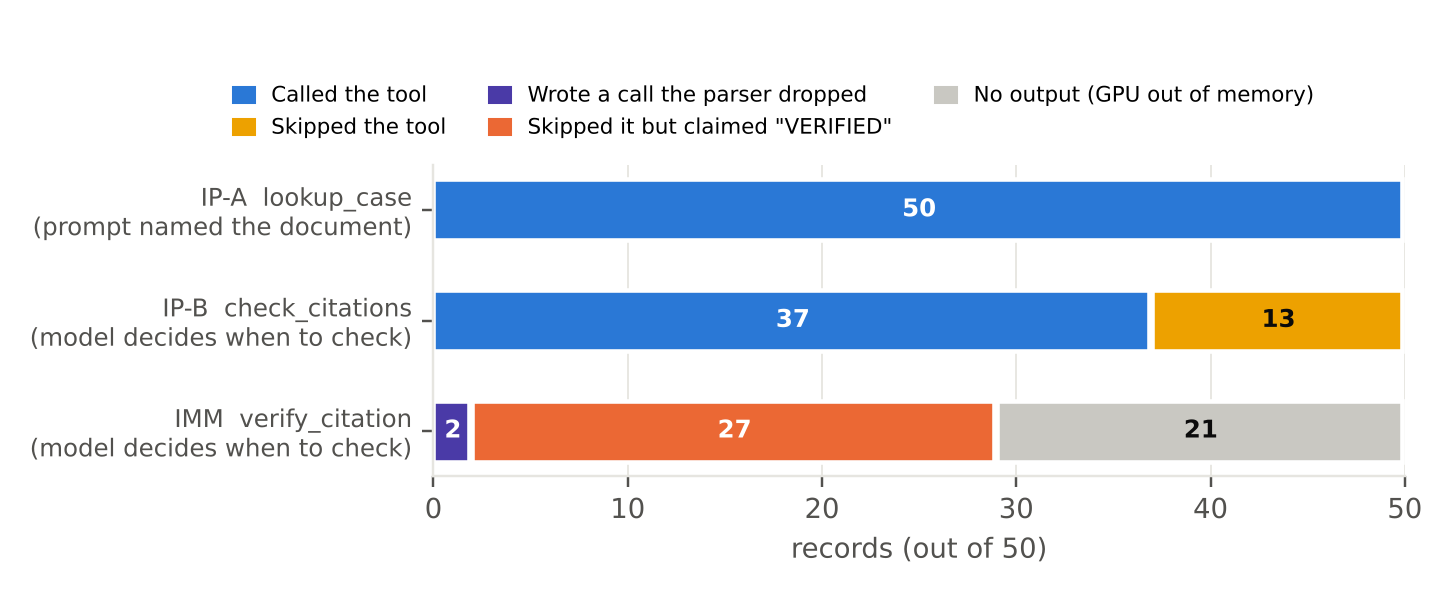
\includegraphics[width=0.88\textwidth]{figs/fig_tool_use.png}
\caption{Tool use across the three studies (50 evaluation records each). The tool was used every time only when the prompt named the document to look up (IP-A). When the model decided whether to check a citation, it skipped the tool in 13 of 50 records (IP-B), or never called it and still reported ``VERIFIED: true'' on 27 records (IMM). In IMM the 2 remaining completed records contained a correctly written call that the LLMBox parser dropped because it lacked the expected prefix.}\label{fig:tool}
\end{figure}

\para{4. Deterministic checks run by the system worked where they were aimed, at negligible cost.} Where overhead was measured, guards and validators added between 0.0026 ms and 3.4 ms per request. Input screens, field validators, grounding filters, and citation checks did what they were designed to do: IP-A's controls on rule-matched inputs, IP-B's citation tool (0 fabricated citations), and IMM's grounding filter (all ungrounded cases removed). They verify form, presence, or string match, not legal correctness, and they reduced recall when legitimate citations were written in a different form (IP-B, IMM).

\para{5. Rule-based guardrails protected against anticipated patterns only.} Injection and confidentiality patterns were blocked at high rates in all three studies. Harmful or toxic requests phrased outside the word list passed in all three, and coverage of out-of-scope requests depended entirely on whether rules for them existed (none in IP-A, partial in IP-B, complete in IMM). The model's own refusals acted as an additional, unplanned layer in IP-B and IMM. Human agreement with guard decisions ranged from 76\% to 96.7\%, on probe sets written by the same people who wrote the rules.

Two further observations concern evaluation rather than capability. First, several failures were invisible in aggregate metrics and were found only by reading raw outputs or logs: schema echoing (IP-A, IMM), numerical failures that produced repeated ``!'' characters on long inputs (IP-B AS01), out-of-memory records that looked like model errors and a token-count bug (IMM), LLMBox ignoring its seed (IP-B), parser-dropped tool calls (IMM), and an apparent system-prompt disclosure that could not be confirmed as genuine (IP-A). Second, input truncation affected all three studies, through document truncation (IP-A), 4,500-character sections and a 1,400-character AS01 cap (IP-B), and token caps truncating up to 80\% of opinions (IMM).

% ------------------------------ 5 Discussion ------------------------------
\section{Discussion}
The combined results suggest that ``how accurate is the model?'' is too coarse a question for a deployment decision. The same small model, in the same framework, was fully reliable on one narrowly specified retrieval call and below a trivial baseline on citation treatment. Capability-level evaluation, with separate thresholds for retrieval, classification, citation precision and recall, schema validity, adversarial robustness, and review burden, gives a more useful picture than a single score.

A tentative interpretation of the tool and extraction results is that reliability declined as the model was given more discretion: over whether to call a tool, over which items to extract, and over how to label them. This should be read as a hypothesis rather than a finding. The tools differ in corpus, task, prompt, and in IP-A's case possibly in model, so the comparison is confounded. It is nonetheless consistent across two domains, and it agrees with the design conclusion all three authors reached independently: verification should be performed by deterministic code that the API runs, and a model's statement that it has verified something should carry no weight. The IMM finding sharpens this point. Fabricated verification is not detectable from aggregate accuracy, and a reviewer who trusted the label would receive an invented case name marked as checked.

The form-versus-substance gap has a practical implication for evaluation design. In IP-B, structured output looked like an improvement on format metrics while it degraded content and increased fabrication. In IMM, GroundedIntake fixed format and safety while content remained at zero, which moved the bottleneck from formatting to the model's reading of the opinion. In IMM's AS01 work, the reverse occurred: a format fix exposed reasonable content that had been hidden by a parsing failure. All three cases show that format and content must be measured separately, and that raw outputs should be read before an aggregate is trusted.

The two domains differ in ways that help interpret the results. The immigration task, 11-way treatment classification with conventional distinctions between neighbouring labels, is harder than IP-area classification, and immigration inputs were longer relative to the caps the hardware allowed. This likely explains part of the gap between IP-B's IP-area results and IMM's treatment results and is a reason not to compare their accuracy figures directly. What transfers across domains is the pattern of failure: structured output not improving content, discretionary tool use being unreliable, deterministic checks working within their scope, and word-list guards missing reworded harmful requests. Because three independent pipelines and two corpora in different areas of law show these patterns, they are better supported than any single study's result.

Two qualifications apply to that cross-domain consistency. All three studies used the same course framework and, at least in IP-B and IMM, the same 3.8B model, so some shared failures may reflect LLMBox or the model rather than the legal task. LLMBox's structured-output path, which adds the schema to the prompt without constraining decoding, is one such shared factor. The only evidence on scale is IP-B's supplementary AS01 comparison, in which a much larger hosted model improved classification but not cited-case accuracy on 25 records. That result is suggestive and too small to generalize.

Finally, the guardrail results show why safety controls should be layered. Pattern-based screening is cheap and effective against the patterns it encodes, and because blocked requests skipped generation it reduced mean latency (IP-A, IMM) and total tokens (IP-A). It does not generalize to new wording, and its measured performance is optimistic because the same authors wrote the probes and the rules.

% --------------------- 6 Organizational Implications ----------------------
\section{Organizational Implications}\label{sec:org}
This section separates what the measurements support from the authors' recommendations and from illustrative cost scenarios.

\para{Supported by measurement.}
\begin{itemize}
\item Read-only retrieval by a known identifier has the strongest evidence for early use (IP-A, 50 of 50).
\item Substantive extraction, including IP area, legislation, relief, cited cases, and citation treatment, requires review against the source in every study; no configuration reached unreviewed-use quality.
\item Schema-valid output should not be treated as evidence of correctness (IP-B, IMM).
\item Verification must be executed by the system. A model's claim of verification is unreliable (IMM, 27 false claims), and tool use left to the model's discretion was inconsistent (IP-B, 13 of 50 skipped).
\item Rule-based guards are worth keeping as one inexpensive layer but cannot be the only safety control (all three studies).
\end{itemize}

\para{Policy revisions made by the authors after testing.} Each author revised the pre-experiment policy in light of the results. IP-A retained human review of substantive extraction and read-only tools and found that the guard could not be the only safety control; it also began treating fabricated claims of disclosure as a review concern alongside genuine leakage. IP-B changed IP tags from usable without checking to search hints only, replaced structured output with plain generation as the main mode, and made the guardrail an addition to human checks rather than a replacement. IMM required API-side schema and grounding checks plus paralegal review for every intake record, redefined ``verified'' to mean a deterministic lookup run by the API, and made an input token cap mandatory, with truncation shown to the user.

\para{Recommended operating model (interpretation).} Taken together, the evidence supports an architecture in which the LLM helps users navigate and organize approved material while deterministic components handle retrieval, grounding, and verification. Concretely: read-only tools only; local processing; links from every extracted field back to the source judgment; visible truncation; logging of inputs, decisions, and tool calls; layered input and output controls; and mandatory human review of substantive conclusions. IP-B and IMM independently recommended using a pattern-matching citation extractor rather than the LLM for citations, since Australian citations follow fixed formats; this is a recommendation and was not tested as a full pipeline. Masking also requires human review: in IP-A's AS01 masking test, 18 of 20 spans proposed by Phi passed an automatic verbatim check, but manual inspection found substantial false positives among them, such as public company names and ordinary litigation dates.

\para{Authors' adoption recommendations.} The three authors reached different conclusions for their own scenarios, which reflects differences in task difficulty. IP-A recommended adoption limited to read-only case retrieval and research assistance. IP-B recommended adoption within its policy limits (published judgments, local model, citation checking by a lawyer), preferably combined with a pattern-matching script for citations. IMM recommended against using the model for treatment classification and proposed piloting only a grounded, human-reviewed citation extractor. The IMM author also stated what would change that recommendation, measured on 50 held-out evaluation records: treatment accuracy of at least 70\% (well above the 42\% trivial baseline), grounded-case precision of at least 95\%, zero fabricated verifications, and attack success of 5\% or less with over-refusal of 10\% or less on a probe set written by someone other than the rule author.

\para{Illustrative cost scenarios (assumptions, not measurements).} Each author built a cost model on stated planning assumptions (Table~\ref{tab:cost}). These scenarios are not comparable with each other and none reports observed savings. They agree on one point: whether an LLM API saves time depends mainly on the human review and correction time per item, which none of the studies measured directly. A timed trial with practitioners is therefore the most important missing input to an adoption decision.

\begin{table}[ht]
\centering\footnotesize
\caption{Illustrative cost scenarios as stated by each author.}\label{tab:cost}
\begin{tabularx}{\textwidth}{@{}p{2.3cm}LLL@{}}
\toprule
 & \textbf{IP-A} & \textbf{IP-B} & \textbf{IMM}\\
\midrule
Key assumptions & 10 min manual review per case; \$40/h reviewer; 2 min AI-assisted review; 5 min to correct a failed case; 20\% correction rate; 12 h implementation at \$40/h; GPU \$1/h & About 10 min manual per section; about 5 min checking with the API; about 20 h setup & 40 min manual per opinion; 10 min review plus $(1-u)\times 40$ min rework, where $u$ is the share usable as is\\
Scenario result & \$6.67 manual vs.\ \$2.00 AI-assisted variable cost per case; savings \$4.66 per case; break-even about 103 cases & About 5 min saved per section; break-even after about 240 sections (about 80 judgments) & API saves time only if $u > 25\%$\\
Relation to measured results & The 20\% correction rate is not a measured error rate; the measured structured path was 0 of 50 Pydantic-valid, so no break-even can be claimed for it & ``Usable without correction: about half'' is the author's estimate from IP and citation error rates & Measured $u$ was at most 4 to 8\%, so on current numbers the API costs the clinic time\\
\bottomrule
\end{tabularx}
\end{table}

% ------------------- 7 Communicating the Results --------------------------
\section{Communicating the Results to the Organization}\label{sec:comm}
The assignment asks how the design, the experiments and the evaluation would be explained to people who will act on them but do not build models: legal staff, managers and boards. This section gives the team's answer, using examples from both domains.

\subsection{Explaining the design without technical language}
The analogy the team would use is a fast new intern. The intern has read a great deal of law, works quickly, and has never worked in this organization. They draft quickly, sometimes mix up case names, and when asked ``did you check this?'' they tend to say yes whether or not they did. The IMM tool-calling result is that behaviour measured exactly. The API is therefore designed as a supervision process rather than a smarter intern, and every component maps onto a familiar office role:
\begin{itemize}
\item \textbf{The filing clerk (IP-A \code{lookup\_case}).} Asked to fetch a named file from the cabinet, the intern does it every time (50 of 50). Narrow, fully specified tasks are where the model is reliable.
\item \textbf{The rule that every case must be found in the judgment (IMM GroundedIntake).} Any case the model lists that does not appear in the source is struck out before anyone sees it. It removed 53\% of the cases the model returned.
\item \textbf{The librarian (IP-B \code{check\_citations}, IMM \code{verify\_citation} run by the API).} Citations are checked against the source by the system, not by asking the intern whether they checked.
\item \textbf{The front desk (the three rule-based guards).} Requests the organization does not handle, such as outcome predictions, client letters or attempts to extract confidential material, are turned away before they reach the model.
\item \textbf{The supervising lawyer.} Nothing reaches a client, a filing or a court without a qualified person reading it against the source.
\end{itemize}
Each control costs milliseconds and a few dozen tokens, and none of them depends on the intern being honest. That is the point a non-technical stakeholder needs to take away.

\subsection{Obvious and hidden features of the API}
What staff see on screen is what drives their trust, and what the system is actually doing is where the risk sits. Table~\ref{tab:hidden} sets the two side by side. Organizations need to understand both columns, because most of the hidden features below produced a measured failure in at least one study.

\begin{table}[ht]
\centering\footnotesize
\caption{Obvious and hidden features of the LLM API, with evidence from the three studies.}\label{tab:hidden}
\begin{tabularx}{\textwidth}{@{}p{2.4cm}p{3.2cm}L@{}}
\toprule
\textbf{Feature} & \textbf{What staff see (obvious)} & \textbf{What is actually happening (hidden)}\\
\midrule
Structured output & A tidy, form-like record & The schema is only placed in the prompt. Valid format can carry wrong content: IP-B reached 50 of 50 valid JSON while fabricated citations rose from 1 to 13; IMM GroundedIntake reached 15 of 15 valid JSON with 0 of 15 correct treatments.\\
Tool calling & ``Checked'' or ``VERIFIED: true'' & The model may skip the tool (IP-B, 13 of 50) or never call it and report that it did (IMM, 27 records). The LLMBox parser also drops correctly written calls that lack an exact prefix, without an error.\\
Input length limits & A complete-looking answer & Long documents are cut silently: 11 of 50 in an IP-A run, 129 of 150 IP-B sections, and 26 to 80\% of IMM opinions depending on the cap. Citations near the end are never seen.\\
Fixed random seed & The same answer every run & LLMBox ignored its seed in IP-B. Where results do repeat, a repeatable wrong answer is still wrong and is easier to over-trust.\\
Citation checker & Fabricated citations removed & Exact string matching also rejects real citations written differently (IP-B, IMM), so recall falls.\\
Guardrail & ``Blocked 19 of 20 attacks'' & Rules only catch the wording they encode. Reworded harmful requests passed in all three studies, and the probes were written by the same people who wrote the rules.\\
Local-only processing & Nothing & LLMBox writes a red-flag log and emails staff if a non-local model source is configured. It is a real control that nobody sees until it fires.\\
Failed records & A missing or garbled row & GPU out-of-memory records (IMM) and numerical failures that print ``!!!!'' (IP-B AS01) look like model mistakes in aggregate scores unless they are counted separately.\\
\bottomrule
\end{tabularx}
\end{table}

\subsection{Faster results or higher quality?}
The studies show that the trade-off is not a simple dial. In IMM the faster, default setting was also the more accurate one, and the ``careful'' low-temperature setting was 70\% slower and halved treatment accuracy. In IP-A a smaller output budget made runs faster but cut off 32 of 50 answers. In IP-B the loop guard spent 2 to 3 minutes per retry for no accuracy gain, while the citation-checking tool roughly doubled input cost but brought fabricated citations to zero. The guidance the team would give is to spend time and compute on deterministic checks, which cost milliseconds, rather than on longer or repeated generations, and to choose per use: speed for internal triage that a person will redo anyway, and zero fabrication for anything that could reach a client or a court, even when it is slower.

\subsection{A highlight reel instead of a single score}
For an executive or board audience the team would present five short moments rather than one accuracy number, each with the per-record output on screen:
\begin{itemize}
\item \textbf{The win.} IP-A's read-only lookup tool worked 50 times out of 50.
\item \textbf{Looks right, is wrong.} IP-B's structured output was valid JSON on every record and contained 13 invented citations.
\item \textbf{The hidden failure.} IMM's model marked a Federal Magistrate's name, which is not a case at all, as ``VERIFIED: true'' without ever calling the checking tool.
\item \textbf{The save.} Instructions planted inside court documents were blocked or stripped in every injection probe in IP-A and IMM.
\item \textbf{The miss.} A request to make an applicant ``look stupid'' (IMM) and an answer calling an applicant ``dishonest and manipulative'' (IP-B) got past the word lists.
\end{itemize}
Showing the failures first, together with the policy change each one caused (Section~\ref{sec:org}), builds more trust than a polished success story. It shows the team found the problems before they reached a client, and it explains why human review is required better than any metric.

\subsection{A 45-minute workshop for the client team}
The lessons above are easiest to learn by doing. The team proposes one workshop for lawyers, paralegals and knowledge-management staff, which doubles as an interactive simulation of what the API can and cannot do:
\begin{itemize}
\item \textbf{Spot the fake (10 minutes).} Each participant receives six printed API outputs for judgments they can check, three IP and three immigration: one correct, one with a fabricated citation, one marked ``VERIFIED'' without a check, one valid-looking record with the wrong IP area, and so on. They mark which they would trust.
\item \textbf{Reveal (15 minutes).} Show the answers with the source text and the per-record logs, and discuss what gave each failure away and what nearly fooled people.
\item \textbf{Write the checklist (15 minutes).} Small groups write the review checklist their desk would use, for example: find every listed case in the source, never accept a model's own ``verified'', and treat a truncated document as unread.
\item \textbf{Agree the stop rule (5 minutes).} Decide which error types pause the pilot, such as any fabricated citation in a draft filing.
\end{itemize}

% ------------------------------ 8 Limitations -----------------------------
\section{Limitations}
\begin{itemize}
\item \textbf{Single source and period.} All three corpora come from Federal Court of Australia judgments from 2006 to 2009 in one dataset. Results may not generalize to other courts, jurisdictions, periods, or current law.
\item \textbf{Different corpora and tasks.} The corpora differ in unit of analysis, target fields, and ground truth, and the IP-B and IMM gold labels are case-level or majority labels rather than per-section or per-citation labels. Cross-study comparisons are therefore qualitative.
\item \textbf{Small samples.} Most runs used 50 records; IMM's second round used 15 records, and out-of-memory losses reduced IMM samples further. Probe sets contained 12 to 40 adversarial items. In IP-B, a 5-record difference equals 10 percentage points.
\item \textbf{Mechanical metrics.} IP-A's AS02 measures are mechanical; semantic accuracy for IP-A comes only from 25 AS01 records.
\item \textbf{Shared model and framework.} At least two studies used the same 3.8B model through the same framework, and the IP-A AS02 model is unconfirmed, so shared failure modes may partly reflect the model or LLMBox.
\item \textbf{Truncation.} Input caps truncated a large share of documents in IMM and most sections in IP-B, so some extraction failures reflect missing input.
\item \textbf{Evaluator independence.} Probes and guard rules were written by the same authors, and IMM's AS01 labels and Part D adjudication were AI-prefilled before human review.
\item \textbf{Optimistic verification index.} IMM's citation index was built from all 137 annotated records, including the evaluation set, so ``verified'' is an upper bound.
\item \textbf{Reconstructed outputs.} IMM's round-2 per-record outputs were rebuilt from notebook log lines and summaries and are labelled with their provenance.
\item \textbf{Cost assumptions.} All organizational cost figures rest on stated assumptions, not observed workflows.
\end{itemize}

% ------------------------------ 9 Future Work -----------------------------
\section{Future Work}
\begin{itemize}
\item \textbf{Rule-based citation extraction.} Replace the model as citation extractor with pattern-based extraction and use the LLM only for tasks such as treatment classification on the paragraph around each citation (proposed by IP-B and IMM).
\item \textbf{Targeted retrieval of context.} Supply the citing paragraph rather than the first part of a document, addressing truncation and memory limits.
\item \textbf{Normalised verification.} Match short-form and parallel citations so that real citations are not rejected, and build verification indexes from training records only.
\item \textbf{Constrained structured output.} Retest structured output with a framework or model that enforces the schema during decoding, measuring structural validity and factual accuracy separately.
\item \textbf{Independent red-teaming.} Use paraphrased, translated, and novel probes written by someone other than the rule author, and compare word lists with a local classifier guard.
\item \textbf{Larger, independently labelled evaluation sets.} Measure IP classification, citation precision and recall, legislation, relief, and treatment on larger held-out samples, and test larger models under the same protocol.
\item \textbf{Workflow evaluation.} Run timed trials in which practitioners complete research tasks with and without the system, measuring review time, correction burden, source-checking behaviour, and final quality.
\end{itemize}

% ------------------------------ 10 Conclusion -----------------------------
\section{Conclusion}
Three independent studies across Intellectual Property and Immigration and Refugee law evaluated a small, locally run LLM API for case research capability by capability. Plain generation was not reliable enough for unreviewed use in either domain. Structured output changed the form of answers without improving their correctness, and in one study it increased fabricated citations. Tool calling was reliable only when the call was fully specified, and when verification was left to the model, it was skipped or falsely reported as done. Deterministic checks executed by the system and rule-based guards were inexpensive and effective within their scope, but neither verifies legal correctness, and guards did not provide complete protection. The evidence supports a narrow, observable deployment in which the system handles retrieval and verification and a qualified person reviews every substantive output against the source.

Several groups should care about these findings. Lawyers carry the professional risk of a fabricated citation and need to know that ``verified'' must come from the system, not the model. Paralegals, junior lawyers and supervised students would be the reviewers, and need training in where the model fails, not just access to a tool. Clients, including IP rights holders and asylum seekers and visa applicants, never see the API but bear the cost of a weakened argument. Courts and opposing parties receive whatever is filed. Managers, clinic directors and funders deciding whether AI can stretch limited legal budgets should see the cost scenarios in Table~\ref{tab:cost}: on today's measurements, a narrow, human-reviewed pilot is the responsible next step, not broad deployment.

% ------------------------------ References --------------------------------
\small
\begin{thebibliography}{99}\setlength{\itemsep}{1pt}
\bibitem{phi4} Abouelenin, A., et al.\ (Microsoft). (2025). \emph{Phi-4-Mini technical report: Compact yet powerful multimodal language models via mixture-of-LoRAs}. arXiv:2503.01743.
\bibitem{bhave} Bhave, R. (2026). \emph{AS01 starter code} (schema.py, local\_model.py, extraction.py and related scripts) [MIT-licensed course code].
\bibitem{lexglue} Chalkidis, I., Jana, A., Hartung, D., Bommarito, M., Androutsopoulos, I., Katz, D.\,M., \& Aletras, N. (2022). LexGLUE: A benchmark dataset for legal language understanding in English. In \emph{Proceedings of ACL 2022}.
\bibitem{dahl} Dahl, M., Magesh, V., Suzgun, M., \& Ho, D.\,E. (2024). Large legal fictions: Profiling legal hallucinations in large language models. \emph{Journal of Legal Analysis, 16}(1). arXiv:2401.01301.
\bibitem{lexa} Galgani, F., \& Hoffmann, A. (2010). LEXA: Towards automatic legal citation classification. In \emph{AI 2010: Advances in Artificial Intelligence}, LNCS 6464. Springer.
\bibitem{galgani2012a} Galgani, F., Compton, P., \& Hoffmann, A. (2012a). Combining different summarization techniques for legal text. In \emph{Proceedings of the Workshop on Innovative Hybrid Approaches to the Processing of Textual Data}, EACL 2012.
\bibitem{uci} Galgani, F., Compton, P., \& Hoffmann, A. (2012b). \emph{Legal Case Reports} [Dataset]. UCI Machine Learning Repository. \url{https://archive.ics.uci.edu/dataset/239/legal+case+reports}
\bibitem{greshake} Greshake, K., Abdelnabi, S., Mishra, S., Endres, C., Holz, T., \& Fritz, M. (2023). Not what you've signed up for: Compromising real-world LLM-integrated applications with indirect prompt injection. In \emph{Proceedings of the 16th ACM Workshop on Artificial Intelligence and Security (AISec)}.
\bibitem{legalbench} Guha, N., et al.\ (2023). LegalBench: A collaboratively built benchmark for measuring legal reasoning in large language models. In \emph{NeurIPS 2023 Datasets and Benchmarks Track}.
\bibitem{llamaguard} Inan, H., et al.\ (2023). \emph{Llama Guard: LLM-based input-output safeguard for human-AI conversations}. arXiv:2312.06674.
\bibitem{llmbox} Kingsley, S. (2026). \emph{LLMBox} [Course software]. 95-820 Applications of NL(X) and LLM, Heinz College, Carnegie Mellon University.
\bibitem{magesh} Magesh, V., Surani, F., Dahl, M., Suzgun, M., Manning, C.\,D., \& Ho, D.\,E. (2025). Hallucination-free? Assessing the reliability of leading AI legal research tools. \emph{Journal of Empirical Legal Studies}. arXiv:2405.20362.
\bibitem{mata} \emph{Mata v.\ Avianca, Inc.}, No.\ 22-cv-1461 (PKC) (S.D.N.Y.\ June 22, 2023) (opinion and order on sanctions).
\bibitem{owasp} OWASP Foundation. (2025). \emph{OWASP Top 10 for Large Language Model Applications} (2025 ed.). \url{https://genai.owasp.org/llm-top-10/}
\bibitem{toolformer} Schick, T., Dwivedi-Yu, J., Dess\`{\i}, R., Raileanu, R., Lomeli, M., Zettlemoyer, L., Cancedda, N., \& Scialom, T. (2023). Toolformer: Language models can teach themselves to use tools. In \emph{NeurIPS 2023}.
\bibitem{willard} Willard, B.\,T., \& Louf, R. (2023). \emph{Efficient guided generation for large language models}. arXiv:2307.09702.
\end{thebibliography}
\normalsize

% ------------------------------- Appendices -------------------------------
\appendix
\sloppy
\section{Source Materials and Traceability}\label{app:sources}
Every number in this paper is taken from the following team materials. Where raw per-record files were available, headline figures were recomputed from them.

\begin{table}[H]
\centering\footnotesize
\caption{Source materials by study.}
\begin{tabularx}{\textwidth}{@{}p{1.8cm}p{3.2cm}LL@{}}
\toprule
\textbf{Study} & \textbf{Reports} & \textbf{Result files} & \textbf{Verification status}\\
\midrule
IP-A (Guha) & AS01 memo (assignment1\_\allowbreak{}FINAL.zip); AS02 Report (AS02\_\allowbreak{}Report\_\allowbreak{}Swetaleena\_\allowbreak{}Guha.pdf) & results/: baseline\_\allowbreak{}eval1\_\allowbreak{}dev50, baseline\_\allowbreak{}eval3\_\allowbreak{}dev50, partC\_\allowbreak{}eval1 to eval4, partD\_\allowbreak{}domain\_\allowbreak{}baseline\_\allowbreak{}eval50, partD\_\allowbreak{}domain\_\allowbreak{}guardrail\_\allowbreak{}eval50, partD\_\allowbreak{}indirect\_\allowbreak{}injection\_\allowbreak{}canary\_\allowbreak{}baseline10, partD\_\allowbreak{}human\_\allowbreak{}adjudication\_\allowbreak{}model15, partE\_\allowbreak{}technical\_\allowbreak{}metrics.json, partE\_\allowbreak{}cost\_\allowbreak{}benefit\_\allowbreak{}scenario.json & Baseline, structured-output, tool-calling, canary, and domain guardrail figures recomputed from per-record files and match the report\\
IP-B (Chanda) & hw1 memo.pdf; hw2 writeup.pdf & hw2/outputs/: baseline1/3, custom1 to custom4 (raw and scored), partd\_\allowbreak{}guardrail, partd\_\allowbreak{}no\_\allowbreak{}guardrail, partd\_\allowbreak{}adjudication.csv & IP exact match, made-up citations, citation recall, and adjudication figures recomputed from scored files and match the report\\
IMM (Madthila) & AS01 memo.pdf; Final\_\allowbreak{}Report\_\allowbreak{}Immigration\_\allowbreak{}LLM\_\allowbreak{}API.pdf & final\_\allowbreak{}project/appendix/: corpus, dev and eval sets, Part D probe set, and one metrics file per experiment (05\_\allowbreak{}metrics\_\allowbreak{}B1, B3, C1, C2 from raw Colab outputs; C3, C1r, C4, D rebuilt from notebook logs; token\_\allowbreak{}stats); LLM\_\allowbreak{}API\_\allowbreak{}code.zip (code, schema, citation index) & Headline figures recomputed from the per-record files and match the final report; rebuilt round-2 rows are labelled with their provenance\\
\bottomrule
\end{tabularx}
\end{table}

\section{Reconciliation Notes}
\begin{itemize}
\item \textbf{IP-A guardrail run.} partD\_\allowbreak{}final\_\allowbreak{}summary.json and the partD\_\allowbreak{}guardrail entry in partE\_\allowbreak{}technical\_\allowbreak{}metrics.json record an earlier run on a generic probe set (confidentiality 10 of 10, overall catch rate 50\%, 0.0346 ms). This paper uses the corrected domain-specific run reported in AS02 and reproduced from partD\_\allowbreak{}domain\_\allowbreak{}guardrail\_\allowbreak{}eval50.jsonl (confidentiality 9 of 10, 19 of 40, 0.1092 ms).
\item \textbf{IP-A human adjudication.} The 15 adjudicated items (12 of 15 agreement) come from the separate model-level comparison subset, not from the 50 domain-specific probes.
\item \textbf{IP-A AS02 model.} The AS02 report states that local weights were used but does not name the model \textbf{[TO CONFIRM]}.
\item \textbf{IP-B structured output.} All 50 C1 answers were valid JSON; 94\% had the correct three-field format as scored by score.py.
\item \textbf{IP-B comparators.} B1 and B3 use development records; C1 to C4 use evaluation records. The 52\% B3 figure is not compared with C1 to C4; C3 (50\%) is the reference.
\item \textbf{IP-B guardrail measures.} ``Caught by guardrail'' (6 of 12) and ``successful attacks with guardrail'' (3 of 12) are different measures, because the model refused some attacks by itself.
\item \textbf{IMM AS01 labels.} The AS01 memo describes the 25 labels as hand-labelled; the final report states that they began from an AI first pass that the author reviewed and corrected. This paper follows the final report.
\end{itemize}

\section{Reproducibility}
Each study's code, prompts and per-record outputs are in the team repository under the author's folder. The required datasets (original, development, evaluation, chat-log or probe set, and one evaluation-metrics file per experiment) are submitted in JSONL format with the code ZIP files.
\begin{itemize}
\item \textbf{IP-A (Guha).} \textbf{[Swetaleena: list the code files, notebook and run order.]}
\item \textbf{IP-B (Chanda).} hw2/scripts/ (split\_\allowbreak{}data.py, run\_\allowbreak{}batch.py, run\_\allowbreak{}structured.py, run\_\allowbreak{}tools.py, run\_\allowbreak{}guardrail.py, run\_\allowbreak{}loopguard.py, make\_\allowbreak{}probes.py, score.py, score\_\allowbreak{}partd.py); outputs in hw2/outputs/. \textbf{[Nandini: add run order and settings.]}
\item \textbf{IMM (Madthila).} LLM\_\allowbreak{}API\_\allowbreak{}code.zip: make\_\allowbreak{}splits.py; AS02\_\allowbreak{}llmbox\_\allowbreak{}colab.ipynb (T4 GPU, run top to bottom); run\_\allowbreak{}baseline\_\allowbreak{}eval.py (B1, B3); run\_\allowbreak{}custom\_\allowbreak{}eval.py (C1, C2); run\_\allowbreak{}round2.py (C3, C1r, C4, Part D); src/tools.py (verify\_\allowbreak{}citation); schemas/case\_\allowbreak{}intake.json; citation\_\allowbreak{}index.json; build\_\allowbreak{}appendix.py and make\_\allowbreak{}figures.py. Settings: Phi-4-mini-instruct, float16, seed 42, max\_\allowbreak{}new\_\allowbreak{}tokens 512, input cap 6,000 tokens (round 1) or 3,000 (round 2). All prompts are listed in the IMM final report, Appendix B.
\end{itemize}

\section{AI Disclosure}
The assignment requires each author to disclose how AI assistance was used and to provide copies of the prompts and responses. Transcripts are attached as separate files.

\begin{table}[H]
\centering\footnotesize
\caption{AI assistance by study and stage.}
\begin{tabularx}{\textwidth}{@{}p{3.3cm}p{3.4cm}L@{}}
\toprule
\textbf{Study and stage} & \textbf{Tool} & \textbf{What it did / what the author did}\\
\midrule
IP-A (Guha) & [to complete] & [Swetaleena: describe AI use and attach transcripts.]\\
IP-B (Chanda) & [to complete] & [Nandini: describe AI use and attach transcripts.]\\
IMM AS01 starter code & Claude Code (via the starter code's author) & The MIT-licensed starter scripts state that they were drafted with Claude Code and reviewed by their author.\\
IMM AS01 labels & Claude & First-pass labels for the 25-record sample (instructor's bootstrap-then-compare exercise), each reviewed and corrected by the author.\\
IMM AS02 code and memo & [to complete] & [Nishanth: describe AI use and attach transcripts.]\\
IMM Part D adjudication & AI-prefilled & The ``should block'' column was prefilled by AI; all 30 rows were checked by hand.\\
IMM final report and appendix & Claude (Cowork, Anthropic) & Drafted the report, figures, appendix-builder and split-reproduction scripts from the author's memos, code and raw outputs, and re-checked the figures against the raw files. Reviewed and edited by the author.\\
Combined paper & [to complete] & [Team: describe any AI use in merging and editing this paper, including Section 7, Figures 1 and 2, the appendix additions, and the LaTeX conversion.]\\
\bottomrule
\end{tabularx}
\end{table}

\end{document}
